\documentclass[a4paper]{article}

% Language and font encodings
\usepackage[english]{babel}
\usepackage[utf8x]{inputenc}
\usepackage[T1]{fontenc}
\usepackage[a4paper,top=3cm,bottom=2cm,left=3cm,right=3cm,marginparwidth=1.75cm]{geometry}
\usepackage{titling}
\usepackage{amsmath}
\usepackage{titlesec}
\usepackage{graphicx}
\usepackage{tabularx}
\usepackage[colorinlistoftodos]{todonotes}
\usepackage[colorlinks=true, allcolors=blue]{hyperref}
\usepackage{fancyhdr}
\usepackage{wrapfig}
\usepackage{subcaption}

\graphicspath{{images/}}

\title{Cosmology Assignment 3}
\author{Daniel Herman: daniel.herman@astro.uio.no}

\begin{document}

\begin{titlepage}
\maketitle
\end{titlepage}

(Code included for exercises 1 and 2 at \url{https://github.com/hermda02/CosmologyAssignment3})\\

\noindent \textbf{Exercise 1.}
Numerical calculations were done with code included at the above github address.\\
i) To find the mean mass per particle, we assume that the medium is highly ionized. Therefore, for each hydrogen atom, the mass is split between the nucleus and the electron. We treat the helium similarly. So we have

\begin{align*}
\mu = \dfrac{<m>}{m_p} = \dfrac{1}{2X+3/4Y}
\end{align*}
Where $X$ is the amount of hydrogen and $Y$ is the amount of helium.
\begin{align*}
\dfrac{1}{\mu} = 2X + 3/4Y
\end{align*}
Using $X = 0.76, Y = 0.24$, we arrrive at $\mu = 0.588$.

ii) The Jeans' mass is derived from the virial theorem:
\begin{align*}
2K = |U| \Rightarrow 3kTN = \dfrac{3GM^2}{5R}, N = \dfrac{M}{\mu*m_p}\\
\dfrac{3kTM}{\mu m_p} = \dfrac{3GM^2}{5R} \Rightarrow \dfrac{3kT}{\mu m_p} = \dfrac{4 \pi GR^3 \rho}{5R}\\
R_J = \sqrt{\dfrac{15kT}{4 \pi G \mu m_p \rho}}
\end{align*}
Using $\rho = \rho_{crit,0}\Omega_{b,0}(1+z)^3$,
\begin{align*}
R_J =& \sqrt{\dfrac{15kT}{4 \pi G \mu m_p \rho_{crit,0}\Omega_{b,0}}}(1+z)^{-3/2}\\
=& 7.787*10^{19} {\rm km} (1+z)^{-3/2}
\end{align*}
So the wave number $k$ is $k = 2\pi / R_J = 8.07*10^{-20}{\rm km^{-1}}(1+z)^{3/2}$\\
iii) The velocity width depends on redshift: $v = HR_J = H_0R_J\sqrt{\Omega_{\Lambda}+\Omega_M(1+z)^3} $\\

\begin{table}[h]
\centering
\begin{tabular}{c | c}
Redshift ($z$) & velocity width\\
\hline
\hline
0 & 171.089\\
1 & 75.986\\
2 & 57.055\\
3 & 48.302\\
4 & 42.843\\
5 & 38.965\\
\end{tabular}
\end{table}

iv) The finite width of the Ly$\alpha$ extinction profile causes absorption features to broaden over redshift as a result of the velocity widths shown in part iii).\\
v) $m = \mu m_p = 0.588{\rm amu} = 9.8196*10^{-25}{\rm g}$
\begin{align*}
v_{TH} = \sqrt{\dfrac{2kT}{m}} = 16.765 {\rm km/s}
\end{align*}
Thus the thermal broadening is far smaller than the Jeans length of the IGM.\\
\clearpage
\noindent \textbf{Exercise 2.}
\begin{figure}[h]
\centering
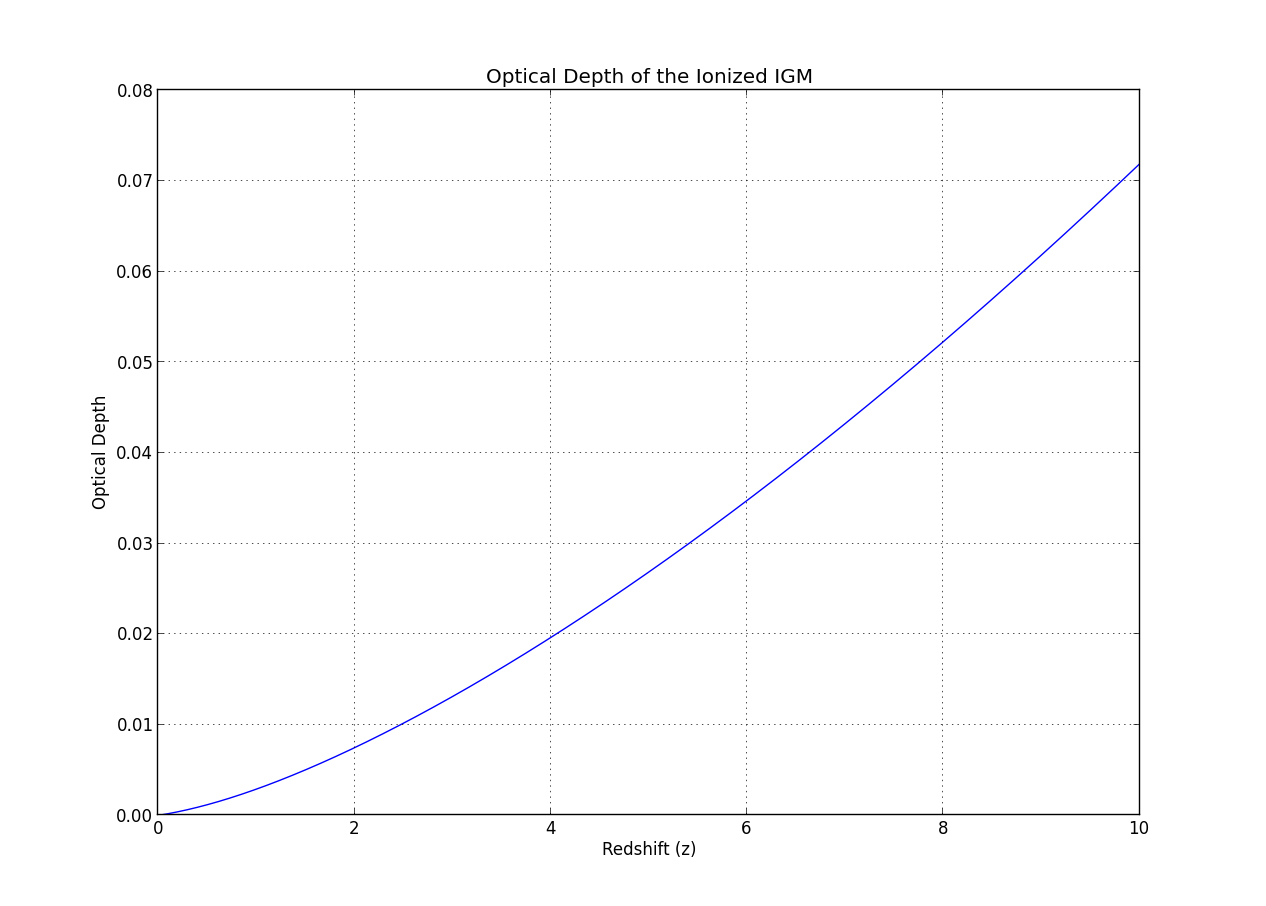
\includegraphics[scale=0.5]{exercise2cosmo3}
\caption{Optical depth of the ionized IGM as a function of redshift.}
\end{figure}

\noindent \textbf{Exercise 3.}\\
i) $\rho(r) = \dfrac{A}{r^2}$, $A = \dfrac{k_B T}{2 \pi G M_{DM}}$\\
\begin{align*}
-\dfrac{k_BT}{M_{DM}r^2}\dfrac{d}{dr}r^2\dfrac{d}{dr}\ln \rho =& 4 \pi G \rho(r)\\
-\dfrac{k_BT}{M_{DM}r^2}\dfrac{d}{dr}r^2 \big[\dfrac{1}{\rho}\dfrac{d\rho}{dr}\big] =& \dfrac{4 \pi G k_B T}{2 \pi G M_{DM}r^2}\\
-\dfrac{k_BT}{M_{DM}r^2}\dfrac{d}{dr}(-2r) =& \dfrac{2k_BT}{M_{DM}r^2}\\
\dfrac{2k_BT}{M_{DM}r^2} =& \dfrac{2k_BT}{M_{DM}r^2}
\end{align*}

\noindent ii) We assume spherical symmetry:
\begin{align*}
\dfrac{\nabla p}{\rho} = - \nabla \phi
\Rightarrow \dfrac{dp}{dr}\dfrac{1}{\rho} = -\dfrac{GM(<r)}{r^2}
\end{align*}
Where $M = \int_0^r 4 \pi r'^2 \rho(r')dr' = 4 \pi A \int_0^r \dfrac{r'^2}{r'^2}dr' = 4 \pi A r = \dfrac{2k_BT}{GM}r$.\\ So the R.H.S. becomes $-\dfrac{2k_BT}{M_{DM}r}$ \\
\clearpage
\noindent For the L.H.S:
\begin{align*}
p = \dfrac{\rho k_BT}{M_{DM}} = \dfrac{k_BT}{M_{DM}}(\dfrac{A}{r^2}),
\dfrac{dp}{dr} = -\dfrac{2Ak_BT}{M_{DM}r^3}
\end{align*}
Multiplying both sides by $\rho$,
\begin{align*}
-\dfrac{2k_BT}{M_{DM}}\dfrac{A}{r^3} =& - \dfrac{2k_BT}{M_{DM}}\dfrac{\rho}{r}\\
-\dfrac{2k_BT}{M_{DM}}\dfrac{A}{r^3} =& -\dfrac{2k_BT}{M_{DM}}\dfrac{A}{r^3}
\end{align*}

\end{document}